\documentclass[11pt,a4paper]{article}
\usepackage[margin=2.4cm]{geometry}
\usepackage{amsmath,amssymb}
\usepackage{graphicx}
\usepackage{caption}
\usepackage{xcolor}
\usepackage[colorlinks=true,urlcolor=blue,linkcolor=blue]{hyperref}
\usepackage{enumitem}
\usepackage{parskip}
\setlist{itemsep=2pt,topsep=3pt}

\newcommand{\rd}{\dot r}
\newcommand{\vd}{\dot v}

\begin{document}

\begin{flushleft}
{\Large\bfseries Reproducing the NMM2 PING bifurcation (Eq.~7.9 / Fig.~7.3)}\\[4pt]
{\normalsize for the TI envelope-demodulation note TN0484}\\[8pt]
\textbf{To:} Raul de Palma \qquad \textbf{From:} Giulio Ruffini \qquad
\textbf{Re:} Rosetta Stone NMM2-PING \\
\textbf{Ask:} the exact synaptic kernel / gains, and the source code (AUTO-07P and/or a
time integrator) used for Fig.~7.3.
\end{flushleft}

\hrule
\medskip

\section{Context}
For TN0484 we want the \textbf{NMM2 PING} as a third model---after a single Jansen--Rit
column and the LaNMM---demonstrating the same mechanism: a weak amplitude-modulated (AM)
electric field $I(t)=p+\lambda E(t)$ driven into the excitatory current is demodulated by
the exact quadratic $v^2$ term and resonantly amplified near a Hopf bifurcation (read out
as a lock-in at the envelope frequency over a $(\Delta f, I)$ plane). For the resonance
claims to be quantitatively honest we need the PING model to be \emph{faithful} (correct
Hopf locations and gamma frequency). We reconstructed it from the Rosetta Stone but our
reconstruction does \textbf{not} reproduce your published bifurcation diagram (Fig.~7.3),
so we would rather start from your exact equations/code.

\section{Target: the published PING bifurcation (Fig.~7.3, Eq.~7.9)}
The diagram shows, as the excitatory input $I$ increases: a saddle-node near $I\approx-1$;
a lower supercritical Hopf $\mathrm{HB}^+\approx 1$; a \textbf{large gamma limit cycle}
peaking at $r\approx0.53$ near $I\approx 11$; an upper $\mathrm{HB}^+\approx 68$; and a
stable focus outside. Parameters (Table~A.1, NMM2-PING), with $I\in[-20,75]$:
\[
\bar\eta_e=\bar\eta_i=0,\quad
J_{ee}=J_{ei}=J_{ie}=1,\ J_{ii}=2,\quad
\tau_e=15,\ \tau_a=10,\ \tau_i=7.5,\ \tau_g=2.5,\quad
\Delta_e=\Delta_i=1 .
\]
\begin{figure}[h]
\centering
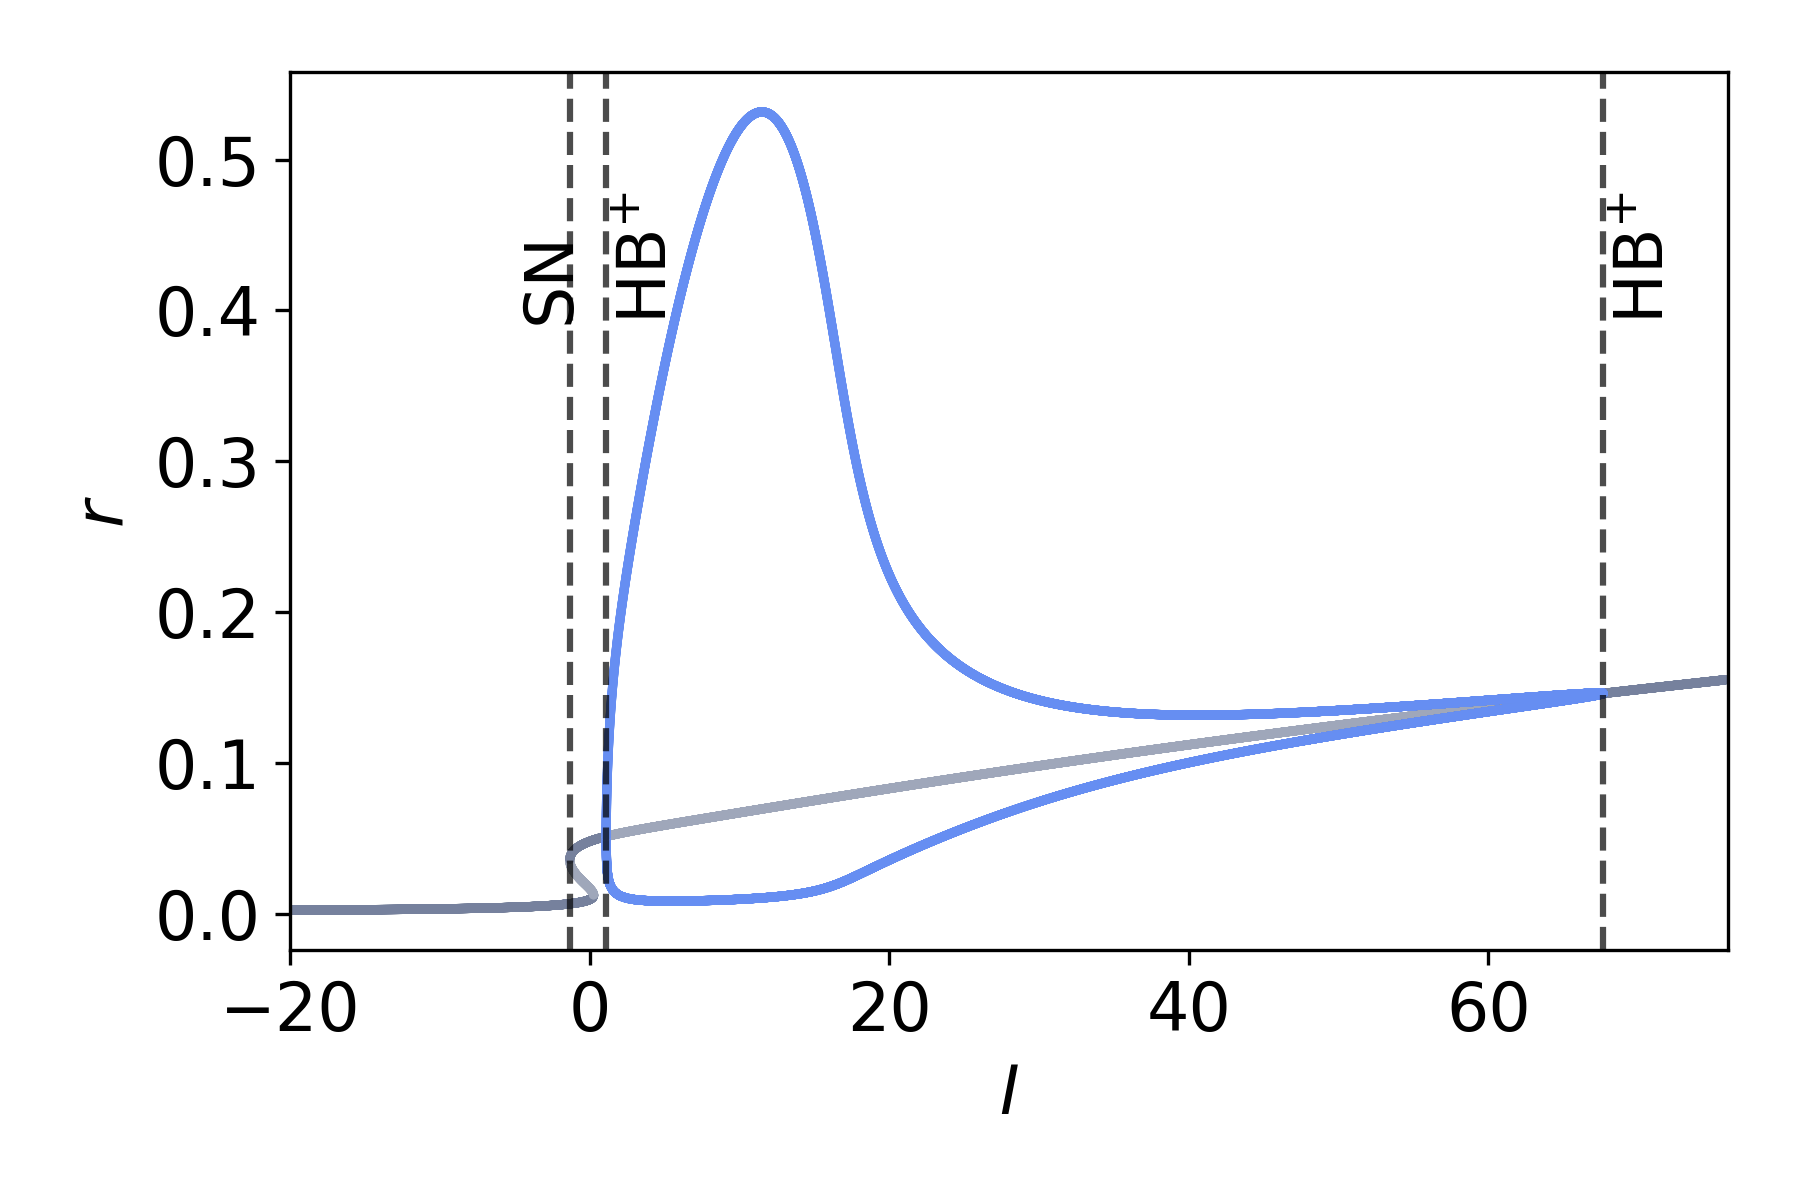
\includegraphics[width=0.62\textwidth]{fig73_ping_bifurcation.png}
\caption*{\small Rosetta Stone, Fig.~7.3 (reproduced): NMM2-PING bifurcation in the
excitatory input $I$. Grey = fixed points (dark stable, light unstable); blue = limit-cycle
max/min. Saddle-node near $I\approx-1$, lower $\mathrm{HB}^+\approx1$, gamma limit cycle
peaking $r\approx0.53$ near $I\approx11$, upper $\mathrm{HB}^+\approx68$, stable focus
outside. \emph{This is the target our reconstruction fails to reproduce.}}
\end{figure}

\section{Our (corrected) reading of Eq.~7.9}
We now use the equations exactly as written in Eq.~7.9 --- in particular the $(r,v)$
membrane equations are \textbf{bare} (no $\tau$ on the left-hand side), and the
cross-couplings are the off-diagonal $J$'s, $C_{xy}=J_{ei}$ (I$\to$E), $C_{yx}=J_{ie}$
(E$\to$I), with $J_x=J_{ee}$, $J_y=J_{ii}$:
\begin{align*}
\rd_x &= \Delta_x/\pi + 2 r_x v_x, &
\vd_x &= v_x^2 + \bar\eta_x + J_x s_x - \pi^2 r_x^2 - C_{xy} s_y + I + \hat F_{e;x}, &
s_x &= \hat K_x[r_x],\\
\rd_y &= \Delta_y/\pi + 2 r_y v_y, &
\vd_y &= v_y^2 + \bar\eta_y - J_y s_y - \pi^2 r_y^2 + C_{yx} s_x, &
s_y &= \hat K_y[r_y].
\end{align*}
\emph{Corrections we made after re-reading Eq.~7.9:} we had wrongly divided the membrane
equations by a membrane time $\tau_e/\tau_i$ (there is none in Eq.~7.9), and we confirmed
the $C=J_{\text{off-diagonal}}$ mapping. With these fixes all four time constants must
live \emph{only} inside the synaptic kernels $\hat K_x,\hat K_y$.

\section{The remaining mismatch}
Even with the bare-membrane form above, a long-settle time-integration:
\begin{itemize}
\item shows \textbf{no clean limit cycle} anywhere in $I\in[-20,75]$;
\item has fixed-point firing rates that climb to $r\approx1$--$2$ (your branch stays
      $\approx0.1$--$0.15$): the scale is $\sim$$10\times$ too high;
\item \textbf{diverges} (overflow) at larger $I$.
\end{itemize}
We suspect the missing pieces are (i) the synaptic kernel definition (a \emph{gain} we are
omitting and/or the rise/decay assignment of the two time constants) and (ii) the
integration method---Fig.~7.3 looks like an AUTO-07P continuation, whereas our explicit
RK4 blows up on the stiff MPR spikes.

\section{Questions}
\begin{enumerate}[label=\textbf{Q\arabic*.}]
\item \textbf{Synaptic kernel $\hat K_x,\hat K_y$.} The review defines $\hat K$ via
      $\gamma^{-1}\!\left(\tau^2\ddot s+2\tau\dot s+s\right)=r$ (equal rise/decay), or
      $(\tau_r,\tau_d)$ for distinct rise/decay. For NMM2-PING:
      \begin{itemize}
      \item what is the synaptic \textbf{gain $\gamma$} for each population? (Table~A.1
            lists the $J$'s, $\tau$'s and $\Delta$ but \emph{no} $\gamma$ --- is
            $\gamma=1$, a JR-style value, or folded into $J$?)
      \item do the two constants map as $\hat K_x=(\tau_e,\tau_a)$ and
            $\hat K_y=(\tau_i,\tau_g)$, and which is rise vs.\ decay? Is the kernel the
            bi-exponential $(\tau_d\,\tfrac{d}{dt}+1)(\tau_r\,\tfrac{d}{dt}+1)\,s=\gamma r$,
            or critically damped with a single $\tau$ (then what are the other two
            constants)?
      \item is the DC gain of $\hat K$ unity ($s\!\to\!r$ at steady state), or $\gamma$?
      \end{itemize}
\item \textbf{Units / scale.} What are the units of $r$ (Fig.~7.3 axis $0$--$0.5$: kHz?
      normalized?) and the time unit, so the gamma frequency lands correctly
      ($\sim$40~Hz)? Our $r$ runs $\sim$$10\times$ high, pointing to a missing
      gain/normalization.
\item \textbf{Source code (the key ask).} Could we get whatever produced Fig.~7.3 --- the
      \textbf{AUTO-07P} files + constants (the table cites
      \url{https://github.com/pclus/auto-tutorial}) and/or a robust \textbf{Python
      time-domain integrator} for Eq.~7.9? With that we can reproduce Fig.~7.3 exactly and
      then add the weak-field AM-drive resonance analysis for TN0484.
\end{enumerate}

\medskip
\hrule
\medskip
\noindent\footnotesize Once we have a faithful PING we will drive $\hat F_{e;x}$ with
$A[1+\cos\Omega t]\cos(\omega_c t)$ and read the lock-in of $r_x$ at $\Omega$ over
$(\Delta f, I)$, showing forced resonance below the Hopf and entrainment within the cycle
--- the gamma analogue of the JR/LaNMM alpha results already in TN0484.

\end{document}
